\documentclass[a4paper,11pt]{article}

\title{Statistical Inference of Discretely Observed Compound Poisson Processes and Related Jump Processes}
\author{Suraj Shah}

\usepackage{amsmath}
\usepackage{amssymb}
\usepackage{amsfonts}
\usepackage{bbm}

\usepackage{amsthm}
\usepackage{cleveref}

\usepackage{graphicx}
\graphicspath{ {./plots/} }

\theoremstyle{theorem}
\newtheorem{thm}{Theorem}
\newtheorem{lem}{Lemma}[section]
\crefname{lem}{Lemma}{Lemmas}
\newtheorem{prop}{Proposition}[section]
\newtheorem*{trapezoid}{Trapezoid Rule}
\newtheorem*{fft}{Fast Fourier Transform}

\theoremstyle{definition}
\newtheorem{defn}{Definition}[section]

\providecommand{\E}{\mathbb{E}}

\begin{document}

\maketitle

\begin{abstract}

\end{abstract}

\pagebreak

\tableofcontents

\pagebreak

\section{Introduction}

\begin{defn}[Counting Process]
A \textit{counting process} is a stochastic process $\{ N(t) : t \geq 0 \}$ with values that are non-negative, integer and non-decreasing i.e. $\forall s,t \geq 0 : s \leq t$ :

\begin{enumerate}

\item $N(t) \geq 0$,
\item $N(t)\in \mathbb{N}$,
\item $N(s) \leq N(t)$.

\end{enumerate}

\end{defn}

\begin{defn}[Poisson Process]
A \textit{Poisson process with intensity $\lambda$} is a counting process $\{ N(t) : t \geq 0 \}$ with the following properties:

\begin{enumerate}

\item $N(0) = 0$,
\item It has independent increments i.e. $\forall n \in \mathbb{N}: 0 \leq t_{1} \leq t_{2} \leq \dotsb \leq t_{n}$, $N(t_{n}) - N(t_{n-1}), N(t_{n-1}) - N(t_{n-2}), \dotsc , N(t_{1})$ are independent,
\item The number of occurrences in any interval of length t is a Poisson random variable with parameter $\lambda t$ i.e. $ \forall s,t : s \leq t$, $N(t) - N(s) \sim {\rm Poisson}(\lambda (t-s))$.

\end{enumerate}

\end{defn}

\begin{lem}
A Poisson process with intensity $\lambda$ has exponentially distributed inter-arrival times with rate $\lambda$.  
\end{lem}

\begin{defn}[Compound Poisson Process] Let ${N(t) : t \geq 0}$ be a d-dimensional Poisson process with intensity $\lambda$. 

Let $Y_{1}, Y_{2}, \dotsc$ be a sequence of i.i.d random variables taking values in $\mathbb{R}^{d}$ with common distribution $F$.

Also assume that the $Y_{i}$'s are independent of the Poisson process $\{N(t) : t \geq 0 \}$.

Then, a \textit{Compound Poisson process (CPP)} is a stochastic process $\{ X(t) : t \geq 0 \}$ such that
\[
X(t) = \sum_{i=1}^{N(t)} Y_{i}
\]
where, by convention, we take $X(t) = 0$ if $N(t) = 0$.

\end{defn}

Suppose we take discrete observations of a CPP i.e. we consider $X(\Delta), X(2\Delta), \dotsc$ where ${X(t) : t \geq 0}$ is a CPP. We want to estimate $F$. Note that the jump size $X(n\Delta) - X((n-1)\Delta)$ is equivalent in distribution to a Poission random sum of intensity $\Delta$:
\begin{align*}
X(n\Delta) - X((n-1)\Delta) &= \sum_{i=1}^{N(n\Delta)}{Y_{i}} - \sum_{i=1}^{N((n-1)\Delta)}{Y_{i}} \\
= \sum_{i=1}^{N(n\Delta) - N((n-1)\Delta)}{Y_{i}} \\
=^{d} \sum_{i=1}^{N}{Y_{i}}
\end{align*}
where $N \sim {\rm Poisson}{(\Delta)}$

\section{Spectral Approach}

Now we have formulated the problem, we visit some methods for estimating the unknown density $f$. Since adding a Poisson number of $Y$'s is referred to as compounding, much of the literature refers to the problem of recovering density $f$ of $Y$'s from observations of $X$ as decompounding.

The approach of decompounding was famously proposed by Buchmann and Gr\"{u}bel to estimate the density $f$ for discrete and continuous cases of the distribution $F$ of the $Y$'s.

Van Es built on this idea for fixed sampling rate $\Delta = 1$ using the L\'{e}vy - Khintchine formula. We explain the idea behind this method and show its strength through various examples.

\subsection{Van Es}

\subsubsection{Construction of Density Estimator via suitable inversion of characteristic functions}

We first note the following property:

\begin{prop}
For Poisson random sum $X$, the characteristic function of $X$, denoted by $\phi_{X}$, is given by $\phi_X(t) = \mathbb{E}e^{itX} = e^{-\lambda + \lambda \phi_{f}(t)}$ 
\end{prop}

\begin{proof}
\begin{align*}
\phi_{X}(t) &= \E e^{itX} \\
          &= \E \left[ \exp\left(it\sum_{i=1}^{N(\lambda)}{Y_{i}}\right)\right] \\
          &= \E \left[ \prod_{i=1}^{N(\lambda)}{\exp(itY_{i})} \right] \\
          &= \E \left[ \E \left[ \prod_{i=1}^{N(\lambda)}{\exp(itY_{i})} \middle| N(\lambda) \right] \right] \\
          &= \E \left[ \prod_{i=1}^{N(\lambda)}{\E \left[ \exp(itY_{1}) \;\middle|\; N(\lambda) \right]} \right] & \text{(by i.i.d assumption of the } Y_{i}\text{'s)}  \\
          &= \E \left[ \prod_{i=1}^{N(\lambda)}{\phi_{f}(t)} \right] & \text{(}Y_{1} \text{ and } N(\lambda) \text{ are independent)} \\
          &= \E \left[ \exp(N(\lambda) \ln\phi_{f}(t)) \right] \\
          &= \exp(\lambda(e^{\ln\phi_{f}(t)} - 1)) & \text{(MGF of a Poisson random variable)} \\
          &= e^{-\lambda + \lambda \phi_{f}(t)}
\end{align*}
\end{proof}

We can rewrite $\phi_{X}(t)$ as:

\begin{align}
\phi_{X}(t) &= e^{-\lambda}(e^{\lambda \phi_{f}(t)} - 1 + 1) \nonumber \\
		    &= e^{-\lambda} + e^{-\lambda}(e^{\lambda \phi_{f}(t)} - 1) \nonumber \\
		    &= e^{-\lambda} + e^{-\lambda}\frac{e^{\lambda} - 1}{e^{\lambda} - 1}(e^{\lambda \phi_{f}(t)} - 1) \nonumber \\
		    &= e^{-\lambda} + \frac{1 - e^{-\lambda}}{e^{\lambda} - 1}(e^{\lambda \phi_{f}(t)} - 1) \label{eq:charX}
\end{align}

Since a zero jump size provides no additional information on the density $f$, we want to gain information about $X$ conditional on the event that there is at least one jump. Seeing that $X \;|\; N(\lambda) > 0$ has a density is somewhat intuitive, but we provide a proof of this.

\begin{lem}
The random variable $X \;|\; N(\lambda) > 0$ has a density.
\end{lem}
\begin{proof}
By the Radon-Nikodym Theorem, a random variable $X$ has a density if and only if $\mathbb{P}(X \in A) = 0$ for every Borel set $A$ with Lebesgue measure zero.

Suppose that Leb$(A) = 0$. Then
\begin{align*}
\mathbb{P}(X \in A | N(\lambda) > 0)
&= \frac{1}{\mathbb{P}(N(\lambda) > 0)}\sum_{n=1}^{\infty}{\mathbb{P}\left(Y_{1} + \dotsb + Y_{n} \in A, N(\lambda) = n\right)} \\
&= \frac{1}{\mathbb{P}(N(\lambda) > 0)}\sum_{n=1}^{\infty}{\mathbb{P}\left(Y_{1} + \dotsb + Y_{n} \in A\right) \mathbb{P}(N(\lambda) = n)}                                     
\end{align*}
Note that for each $n, Y_{1} + \dotsb + Y_{n}$ has a density so $\mathbb{P}\left(Y_{1} + \dotsb + Y_{n} \in A\right) = 0$. Thus the result follows.

\end{proof}
Let $g$ be the density of $X \;|\; N(\lambda) > 0$. 

Let $\phi_{g}(t) = \E \left[ e^{itX} \;\middle|\; N(\lambda) > 0 \right] = \frac{\E \left[ e^{itX} \mathbbm{1}(N(\lambda) > 0) \right]}{\mathbb{P}(N(\lambda) > 0)}$.

Then
\begin{align*}
\phi_{X}(t) &= \E \left[ e^{itX} \mathbbm{1}(N(\lambda) = 0) \right] + \E \left[ e^{itX} \mathbbm{1}(N(\lambda) > 0) \right] \\
            &= \mathbb{P}(N(\lambda) = 0) + \mathbb{P}(N(\lambda) > 0) \phi_{g}(t) \\
            &= e^{-\lambda} + (1 - e^{-\lambda})\phi_{g}(t)
\end{align*}

Therefore, using (\ref{eq:charX}), we get that
\begin{equation}
\phi_{g}(t) = \frac{1}{e^{\lambda} - 1}(e^{\lambda \phi_{f}(t)} - 1) \label{eq:charg}
\end{equation}

Thus, we can see from this that if we were to obtain an estimator for $\phi_{g}(t)$, then by suitable inversion of the formula in (\ref{eq:charg}), we would obtain an estimator for $\phi_{f}(t)$.

In order to rewrite (\ref{eq:charg}) in terms of $\phi_{f}(t)$, we must be able to invert the complex exponential function since $\phi_{f}(t)$ takes complex values. However, such function is not invertible since it is not bijective: in particular it is not injective as $e^{w + 2 \pi i} = e^{w} \ \forall w \in \mathbb{C}$.

Therefore, we use the following lemmas concerning the distinguished logarithm:

\begin{lem} \label{lma1}
If $h_{1} : \mathbb{R} \to \mathbb{C}$ and $h_{2} : \mathbb{R} \to \mathbb{C}$ are continuous functions such that $h_{1}(0) = h_{2}(0) = 0$ and $e^{h_{1}} = e^{h_{2}}$, then $h_{1} = h_{2}$. 
\end{lem}

\begin{proof}
See Appendix.
\end{proof}

\begin{lem} \label{lma2}
If $\phi : \mathbb{R} \to \mathbb{C}$ is a continuous function such that $\phi(0) = 1$ and $\phi_{g}(t) \neq 0 \ \forall t \in \mathbb{R}$ then there exists a unique continuous function $h : \mathbb{R} \to \mathbb{C}$ with $h(0) = 0$ and $\phi(t) = e^{h(t)}$ for $t \in \mathbb{R}$. 
\end{lem}

\begin{proof}
See Appendix.
\end{proof}

Therefore, for such a function $\phi$ as described in the Lemma, we say that the unique function $h$ is the distinguished logarithm and we denote $h(t) = \text{Log}(\phi(t))$. Note also that for $\phi$ and $\psi$ satisfying the assumptions of the Lemma, we have $\text{Log}(\phi(t)\psi(t)) = \text{Log}(\phi(t)) + \text{Log}(\psi(t))$ as expected.  

Therefore, noting that $\phi(t) = e^{\lambda(\phi_{f}(t) - 1)}$ is a continuous function satisfying $\phi(0) = 1$ and $\phi(t) \neq 0 \ \forall t \in R$, we get that
\begin{align*}
\lambda(\phi_{f}(t) - 1) &= \text{Log}\left(e^{\lambda (\phi_{f}(t) - 1)}\right)& \text{(\cref{lma1})} \\
                         &= \text{Log}\left(e^{-\lambda}\left[(e^{\lambda} - 1)\phi_{g}(t) + 1\right] \right) \\
                         &= -\lambda + \text{Log}\left((e^{\lambda} - 1)\phi_{g}(t) + 1\right)
\end{align*}

Therefore,
\begin{equation} \label{eq:charf}
\phi_{f}(t) = \frac{1}{\lambda}\text{Log}\left((e^{\lambda} - 1)\phi_{g}(t) + 1\right)
\end{equation} 

By Fourier inversion, for integrable $\phi_{f}$ we have
\begin{equation} \label{eq:fourier}
f(x) = \frac{1}{2\pi\lambda}\int_{-\infty}^{\infty}{e^{-itx}\text{Log}\left((e^{\lambda} - 1)\phi_{g}(t) + 1\right)}dt
\end{equation}

This suggests that if we can estimate $\phi_{g}(t)$, then we have an estimate of $f$.

\subsubsection{Kernel density estimators}

We provide the intuition behind choosing our estimator for $g$ on observations of non-zero jump size as a kernel density estimator.

Let $X$ be a random variable with probability density $p$ with respect to the Lebesgue measure on $\mathbb{R}$. The corresponding distribution function is $F(x) = \int_{-\infty}^{x}{p(t)}dt$.

Consider n i.i.d observations $X_{1}, \dotsc , X_{n}$ with same distribution as $X$. The empirical distribution function is given by 
\[
F_{n}(x) = \frac{1}{n}\sum_{i=1}^{n}{I(X_{i} \leq x)}
\]  

By the Strong Law of Large Numbers, since for fixed $x$, $I(X_{i} \leq x)$ are i.i.d , we have that
\[
F_{n}(x) \to \E \left[ I(X_{1} \leq x) \right] = \mathbb{P}(X \leq x) = F(x)
\]
almost surely as $n \to \infty$.

Therefore, $F_{n}(x)$ is a consistent estimator of $F(x)$ for every $x \in \mathbb{R}$. Also note that $p(x) = \frac{\mathrm{d}}{\mathrm{d}x}F(x)$, so for sufficiently small $h > 0$ we can write an approximation
\[
p(x) \approx \frac{F(x+h) - F(x-h)}{2h}
\]
Thus, intuitively we can replace $F$ by our empirical distribution function $F_{n}$ to give us an estimator $\hat{p}_{n}(x)$ of $p(x)$
\begin{align*}
\hat{p}_{n}(x) &= \frac{F_{n}(x+h) - F_{n}(x-h)}{2h} \\
               &= \frac{1}{2nh}\sum_{i=1}^{n}{I(x - h < X_{i} \leq x + h)} \\
               &= \frac{1}{nh}\sum_{i=1}^{n}{K_{0}\left(\frac{x - X_{i}}{h}\right)}
\end{align*}
where $K_{0}(u) = \frac{1}{2}I(-1 < u \leq 1)$.

A simple generalisation is to replace $K_{0}$ by some arbitrary (but well-chosen) integrable function $K : \mathbb{R} \to \mathbb{R}$ such that $\int{K(u)}du = 1$ and $K(u) = K(-u)$ for every $u \in \mathbb{R}$. Such a function $K$ is called a \textit{kernel} and the parameter $h$ is called a \textit{bandwidth} of the estimator
\begin{equation} \label{kde}
\hat{p}_{n}(x) = \frac{1}{nh}\sum_{i=1}^{n}{K\left(\frac{x - X_{i}}{h}\right)}
\end{equation}
We call this estimator a \textit{kernel density estimator}.

Thus, for some kernel $w$ with characteristic function $\phi_{w}$ and observations $Z_{1}, \dotsc , Z_{n}$, we estimate density $g$ by the kernel density estimator
\[
g_{nh}(x) = \frac{1}{nh}\sum_{i=1}^{n}{w\left(\frac{x - Z_{i}}{h}\right)}
\]
Letting $\phi_{\text{emp}}(t) = \frac{1}{n}\sum_{j=1}^{n}{e^{itZ_{j}}}$ be the empirical characteristic function, we get that
\begin{align*}
\phi_{g_{nh}}(t) &= \int_{-\infty}^{\infty}{e^{itx}g_{nh}(x)}dx \\
                 &= \int_{-\infty}^{\infty}{e^{itx}\frac{1}{nh}\sum_{j=1}^{n}{w\left(\frac{x - Z_{j}}{h}\right)}}dx \\
                 &= \frac{1}{n}\sum_{j=1}^{n}{e^{itZ_{j}}}\int_{-\infty}^{\infty}{e^{ithy}w(y)}dy &\left(\text{by the substitution } y = \frac{x - Z_{j}}{h} \right) \\
                 &= \phi_{\text{emp}}(t)\phi_{w}(ht)
\end{align*}

In view of (\ref{eq:fourier}) It is tempting to introduce an estimator $\hat{f}_{nh}$ of $f$

\begin{equation} \label{fnh}
\hat{f}_{nh}(x)= \frac{1}{2\pi\lambda}\int_{-\infty}^{\infty}{e^{-itx}\text{Log}\left((e^{\lambda} - 1)\phi_{\text{emp}}(t)\phi_{w}(ht) + 1\right)}dt
\end{equation}
but this brings two main issues:
\begin{enumerate}
\item In light of \cref{lma2}, we may have some Borel set $A$ with non-zero Lebesgue measure such that $(e^{\lambda} - 1)\phi_{\text{emp}}(t)\phi_{w}(ht) + 1$ is zero for $ t \in A$. The distinguished logarithm is undefined under such sets and thus our estimator of $f$ is undefined in this case.
\item There is no guarantee that the integral is finite. For example,
\[
\phi_{g_{nh}}(t) = \frac{\exp(e^{it}) - 1}{e^{\lambda} - 1}
\]
would give $\hat{f}_{nh}(1)$ to be infinity.
\end{enumerate}

In order to prove asymptotic properties, we must adjust our estimators by bounding $\hat{f}_{nh}$ for each $n$ using a suitable sequence $(M_{n})_{n \geq 1}$. However, for our discussion, we note such limitations and provide simulations for examples where these two cases do not occur.

\subsubsection{Simulation Results}

We note that for $\lambda < \log2$, the distinguished logarithm in (\ref{fnh}) reduces to the principal branch of the logarithm. This is the logarithm whose imaginary part lies in the interval $\left(-\pi, \pi\right]$. We also note, as written above, that bounding $\hat{f}_{nh}$ by a suitable sequence is not needed in practice. Therefore, we can use (\ref{fnh}) to compute our estimator with the principal branch of the logarithm, provided $\lambda < \log 2$.

We use the following kernel $w$ given by
\[
w(t) = \frac{48t(t^{2} - 1)\cos t - 144(2t^{2} - 5)\sin t}{\pi t^{7}}
\]

This kernel has a fairly complicated form but its characteristic function $\phi_{w}(t)$ has a much simpler expression given by
\[
\phi_{w}(t) = (1 - t^{2})^{3}\mathbbm{1}\{|t| < 1\}
\]

We can rewrite (\ref{fnh}) as $\hat{f}_{nh}(x) = \hat{f}_{nh}^{(1)}(x) + \hat{f}_{nh}^{(2)}(x)$ where

\begin{equation} \label{fnh1}
\hat{f}_{nh}^{(1)}(x) = \frac{1}{2\pi\lambda}\int_{0}^{\infty}{e^{-itx}\text{Log}\left((e^{\lambda} - 1)\phi_{\text{emp}}(t)\phi_{w}(ht) + 1\right)}dt 
\end{equation}

\begin{align}
\hat{f}_{nh}^{(2)}(x) &= \frac{1}{2\pi\lambda}\int_{-\infty}^{0}{e^{-itx}\text{Log}\left((e^{\lambda} - 1)\phi_{\text{emp}}(t)\phi_{w}(ht) + 1\right)}dt \nonumber \\
                      &= \frac{1}{2\pi\lambda}\int_{0}^{\infty}{e^{itx}\text{Log}\left((e^{\lambda} - 1)\phi_{\text{emp}}(-t)\phi_{w}(ht) + 1\right)}dt \label{fnh2}
\end{align}
since $\phi_{w}$ is symmetric.
We use a bandwidth of $0.14$. Such a bandwidth is arbitrary and we may use better methods to compute a bandwidth estimator that yields better results. This can be done via cross-validation.

We approximate (\ref{fnh1}) and (\ref{fnh2}) by the Trapezoid Rule:
 
\begin{trapezoid}
Let $\{t_{j}\}_{j=0}^{N-1}$ be a set of $N$ equally spaced values partitioning $[a,b]$, with spacing $\Delta t_{k} = \Delta t = \frac{b-a}{N}$. Then, for integrable function $f$ we get the following approximation
\begin{equation} \label{trap}
\int_{a}^{b}{f(x)dx} \approx \Delta t\left( \frac{f(t_{0}) + f(t_{N-1})}{2} + \sum_{j=1}^{N-2}{f(t_{j})}\right)
\end{equation} 
\end{trapezoid}

We can approximate (\ref{fnh1}) (and similarly (\ref{fnh2})) by computing the integrand from $0$ to some sufficiently large $M$.

We may also allow for (\ref{trap}) to be written as a 'nice' sum in order to compute the Fast Fourier Transform. Thus, we write
\begin{equation}
\int_{a}^{b}{f(t)dt} \approx \Delta t\left(\sum_{j=0}^{N-1}{f(t_{j})}\right)
\end{equation} 

Applying this to (\ref{fnh1}) and (\ref{fnh2}) we get for $t_{j} = j\eta$ for some spacing parameter $\eta$
\begin{equation}
\hat{f}_{nh}^{(1)}(x) \approx \frac{\eta}{2\pi\lambda}\sum_{k=0}^{N-1}{e^{-it_{j}x}\text{Log}\left((e^{\lambda} - 1)\phi_{\text{emp}}(t_{j})\phi_{w}(ht_{j}) + 1\right)},
\end{equation}

\begin{equation}
\hat{f}_{nh}^{(2)}(x) \approx \frac{\eta}{2\pi\lambda}\sum_{k=0}^{N-1}{e^{it_{j}x}\text{Log}\left((e^{\lambda} - 1)\phi_{\text{emp}}(-t_{j})\phi_{w}(ht_{j}) + 1\right)},
\end{equation}

We apply the Fast Fourier Transform to evaluate our functions $\hat{f}_{nh}^{(1)}$ and $\hat{f}_{nh}^{(2)}$ at points $\{x_{k}\}_{k=0}^{N-1}$.

\begin{fft}
Let $\{x_{k}\}_{k=0}^{N-1}$ be a sequence of complex numbers. The Fast Fourier Transform computes the sequence $\{Y_{j}\}_{j=0}^{N-1}$ where
\begin{equation}
Y_{j} = \sum_{k=0}^{N-1}{x_{k}e^{-ij\frac{2\pi k}{N}}}
\end{equation}
The inverse transform is given by
\begin{equation}
Y_{j} = \frac{1}{N}\sum_{k=0}^{N-1}{x_{k}e^{ij\frac{2\pi k}{N}}}
\end{equation}
\end{fft}

Thus, we employ a regular spacing with parameter $\delta$ so that our values $\{x_{k}\}_{k=0}^{N-1}$ evenly spaced and given by
\[
x_{k} = \frac{-N\delta}{2} + \delta k
\]

Thus we have
\begin{equation}
\hat{f}_{nh}^{(1)}(x_{k}) \approx \frac{1}{2\pi\lambda}\sum_{k=0}^{N-1}{e^{-ijk\eta\delta}e^{it_{j}\frac{N\delta}{2}}\psi^{(1)}(t_{j})\eta},
\end{equation}

\begin{equation}
\hat{f}_{nh}^{(2)}(x_{k}) \approx \frac{1}{2\pi\lambda}\sum_{k=0}^{N-1}{e^{ijk\eta\delta}e^{-it_{j}\frac{N\delta}{2}}\psi^{(2)}(t_{j})\eta},
\end{equation}

Therefore, we take $\eta\delta = \frac{2\pi}{N}$ and we apply FFT on the sequence $\left\lbrace e^{it_{j}\frac{N\delta}{2}}\psi^{(1)}(t_{j})\eta \right\rbrace_{j=0}^{N-1}$ to get values for $\hat{f}_{nh}^{(1)}$ and we apply IFFT on the sequence $\left\lbrace e^{-it_{j}\frac{N\delta}{2}}\psi^{(2)}(t_{j})\eta \right\rbrace_{j=0}^{N-1}$ to get values for $\hat{f}_{nh}^{(2)}$.

We take $N$ to be a power of 2 for computational speed up in calculating the Discrete Fourier Transforms and we choose $\eta$ relatively small so that $\delta$ can be relatively larger and so points are relatively separate from one another.

The results for $N = 16384$ and $\eta = 0.01$ based on 1000 observations can be shown in Figure 1.

\begin{figure}[h]
\centering
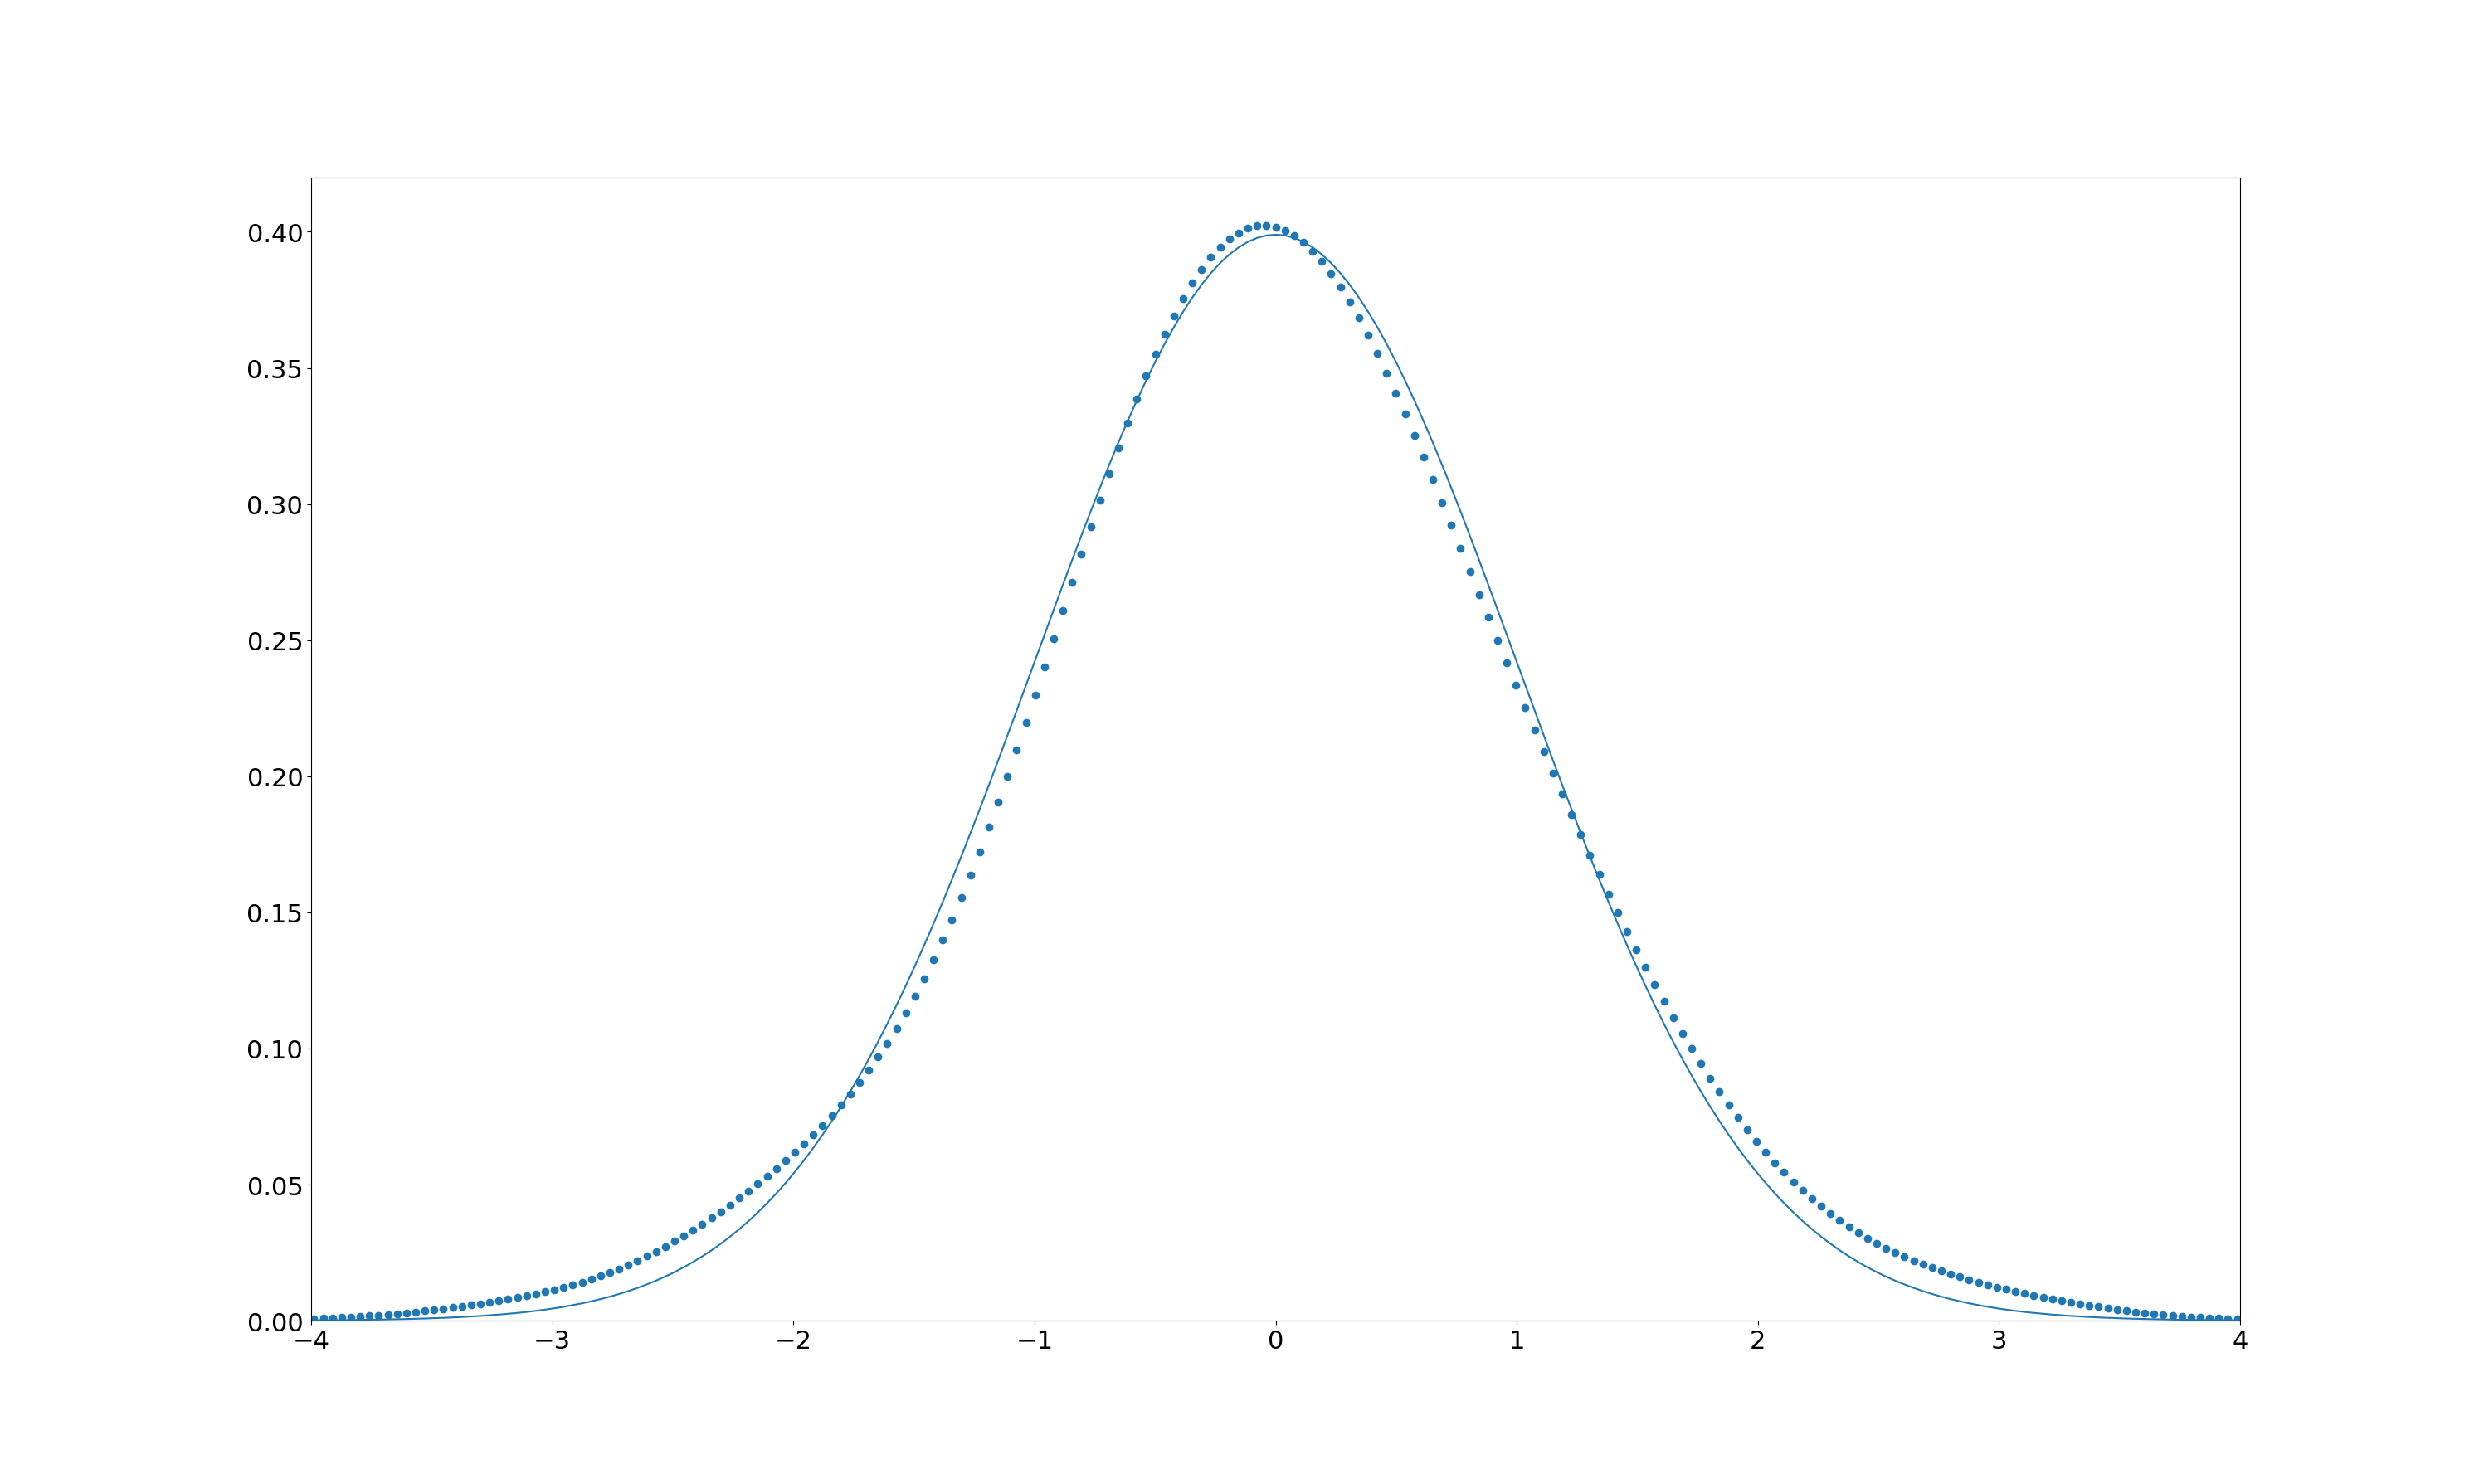
\includegraphics[scale=0.15]{fft_standard_normal.png}
\caption{Density Estimator of Standard Normal}
\label{stdNormal}
\end{figure} 

The second example we consider is the case of $f$ being a mixture of two normal densities
\[
f(\cdot) = \rho_{1}\psi(\cdot;\mu_{1},\sigma_{1}^{2}) + \rho_{2}\psi(\cdot;\mu_{2}, \sigma_{2}^{2}) 
\] 
where $\rho_{1} = \frac{2}{3}, \rho_{2} = \frac{1}{3}, \mu_{1} = 0, \mu_{2} = 3, \sigma_{1}^{2} = 1, \sigma_{2}^{2} = \frac{1}{9}$. We use a bandwidth of 0.1.
\end{document}